% Options for packages loaded elsewhere
\PassOptionsToPackage{unicode}{hyperref}
\PassOptionsToPackage{hyphens}{url}
\PassOptionsToPackage{dvipsnames,svgnames,x11names}{xcolor}
%
\documentclass[
  letterpaper,
  DIV=11,
  numbers=noendperiod]{scrartcl}

\usepackage{amsmath,amssymb}
\usepackage{lmodern}
\usepackage{iftex}
\ifPDFTeX
  \usepackage[T1]{fontenc}
  \usepackage[utf8]{inputenc}
  \usepackage{textcomp} % provide euro and other symbols
\else % if luatex or xetex
  \usepackage{unicode-math}
  \defaultfontfeatures{Scale=MatchLowercase}
  \defaultfontfeatures[\rmfamily]{Ligatures=TeX,Scale=1}
\fi
% Use upquote if available, for straight quotes in verbatim environments
\IfFileExists{upquote.sty}{\usepackage{upquote}}{}
\IfFileExists{microtype.sty}{% use microtype if available
  \usepackage[]{microtype}
  \UseMicrotypeSet[protrusion]{basicmath} % disable protrusion for tt fonts
}{}
\makeatletter
\@ifundefined{KOMAClassName}{% if non-KOMA class
  \IfFileExists{parskip.sty}{%
    \usepackage{parskip}
  }{% else
    \setlength{\parindent}{0pt}
    \setlength{\parskip}{6pt plus 2pt minus 1pt}}
}{% if KOMA class
  \KOMAoptions{parskip=half}}
\makeatother
\usepackage{xcolor}
\setlength{\emergencystretch}{3em} % prevent overfull lines
\setcounter{secnumdepth}{-\maxdimen} % remove section numbering
% Make \paragraph and \subparagraph free-standing
\ifx\paragraph\undefined\else
  \let\oldparagraph\paragraph
  \renewcommand{\paragraph}[1]{\oldparagraph{#1}\mbox{}}
\fi
\ifx\subparagraph\undefined\else
  \let\oldsubparagraph\subparagraph
  \renewcommand{\subparagraph}[1]{\oldsubparagraph{#1}\mbox{}}
\fi

\usepackage{color}
\usepackage{fancyvrb}
\newcommand{\VerbBar}{|}
\newcommand{\VERB}{\Verb[commandchars=\\\{\}]}
\DefineVerbatimEnvironment{Highlighting}{Verbatim}{commandchars=\\\{\}}
% Add ',fontsize=\small' for more characters per line
\usepackage{framed}
\definecolor{shadecolor}{RGB}{241,243,245}
\newenvironment{Shaded}{\begin{snugshade}}{\end{snugshade}}
\newcommand{\AlertTok}[1]{\textcolor[rgb]{0.68,0.00,0.00}{#1}}
\newcommand{\AnnotationTok}[1]{\textcolor[rgb]{0.37,0.37,0.37}{#1}}
\newcommand{\AttributeTok}[1]{\textcolor[rgb]{0.40,0.45,0.13}{#1}}
\newcommand{\BaseNTok}[1]{\textcolor[rgb]{0.68,0.00,0.00}{#1}}
\newcommand{\BuiltInTok}[1]{\textcolor[rgb]{0.00,0.23,0.31}{#1}}
\newcommand{\CharTok}[1]{\textcolor[rgb]{0.13,0.47,0.30}{#1}}
\newcommand{\CommentTok}[1]{\textcolor[rgb]{0.37,0.37,0.37}{#1}}
\newcommand{\CommentVarTok}[1]{\textcolor[rgb]{0.37,0.37,0.37}{\textit{#1}}}
\newcommand{\ConstantTok}[1]{\textcolor[rgb]{0.56,0.35,0.01}{#1}}
\newcommand{\ControlFlowTok}[1]{\textcolor[rgb]{0.00,0.23,0.31}{#1}}
\newcommand{\DataTypeTok}[1]{\textcolor[rgb]{0.68,0.00,0.00}{#1}}
\newcommand{\DecValTok}[1]{\textcolor[rgb]{0.68,0.00,0.00}{#1}}
\newcommand{\DocumentationTok}[1]{\textcolor[rgb]{0.37,0.37,0.37}{\textit{#1}}}
\newcommand{\ErrorTok}[1]{\textcolor[rgb]{0.68,0.00,0.00}{#1}}
\newcommand{\ExtensionTok}[1]{\textcolor[rgb]{0.00,0.23,0.31}{#1}}
\newcommand{\FloatTok}[1]{\textcolor[rgb]{0.68,0.00,0.00}{#1}}
\newcommand{\FunctionTok}[1]{\textcolor[rgb]{0.28,0.35,0.67}{#1}}
\newcommand{\ImportTok}[1]{\textcolor[rgb]{0.00,0.46,0.62}{#1}}
\newcommand{\InformationTok}[1]{\textcolor[rgb]{0.37,0.37,0.37}{#1}}
\newcommand{\KeywordTok}[1]{\textcolor[rgb]{0.00,0.23,0.31}{#1}}
\newcommand{\NormalTok}[1]{\textcolor[rgb]{0.00,0.23,0.31}{#1}}
\newcommand{\OperatorTok}[1]{\textcolor[rgb]{0.37,0.37,0.37}{#1}}
\newcommand{\OtherTok}[1]{\textcolor[rgb]{0.00,0.23,0.31}{#1}}
\newcommand{\PreprocessorTok}[1]{\textcolor[rgb]{0.68,0.00,0.00}{#1}}
\newcommand{\RegionMarkerTok}[1]{\textcolor[rgb]{0.00,0.23,0.31}{#1}}
\newcommand{\SpecialCharTok}[1]{\textcolor[rgb]{0.37,0.37,0.37}{#1}}
\newcommand{\SpecialStringTok}[1]{\textcolor[rgb]{0.13,0.47,0.30}{#1}}
\newcommand{\StringTok}[1]{\textcolor[rgb]{0.13,0.47,0.30}{#1}}
\newcommand{\VariableTok}[1]{\textcolor[rgb]{0.07,0.07,0.07}{#1}}
\newcommand{\VerbatimStringTok}[1]{\textcolor[rgb]{0.13,0.47,0.30}{#1}}
\newcommand{\WarningTok}[1]{\textcolor[rgb]{0.37,0.37,0.37}{\textit{#1}}}

\providecommand{\tightlist}{%
  \setlength{\itemsep}{0pt}\setlength{\parskip}{0pt}}\usepackage{longtable,booktabs,array}
\usepackage{calc} % for calculating minipage widths
% Correct order of tables after \paragraph or \subparagraph
\usepackage{etoolbox}
\makeatletter
\patchcmd\longtable{\par}{\if@noskipsec\mbox{}\fi\par}{}{}
\makeatother
% Allow footnotes in longtable head/foot
\IfFileExists{footnotehyper.sty}{\usepackage{footnotehyper}}{\usepackage{footnote}}
\makesavenoteenv{longtable}
\usepackage{graphicx}
\makeatletter
\def\maxwidth{\ifdim\Gin@nat@width>\linewidth\linewidth\else\Gin@nat@width\fi}
\def\maxheight{\ifdim\Gin@nat@height>\textheight\textheight\else\Gin@nat@height\fi}
\makeatother
% Scale images if necessary, so that they will not overflow the page
% margins by default, and it is still possible to overwrite the defaults
% using explicit options in \includegraphics[width, height, ...]{}
\setkeys{Gin}{width=\maxwidth,height=\maxheight,keepaspectratio}
% Set default figure placement to htbp
\makeatletter
\def\fps@figure{htbp}
\makeatother

\KOMAoption{captions}{tableheading}
\makeatletter
\makeatother
\makeatletter
\makeatother
\makeatletter
\@ifpackageloaded{caption}{}{\usepackage{caption}}
\AtBeginDocument{%
\ifdefined\contentsname
  \renewcommand*\contentsname{Table of contents}
\else
  \newcommand\contentsname{Table of contents}
\fi
\ifdefined\listfigurename
  \renewcommand*\listfigurename{List of Figures}
\else
  \newcommand\listfigurename{List of Figures}
\fi
\ifdefined\listtablename
  \renewcommand*\listtablename{List of Tables}
\else
  \newcommand\listtablename{List of Tables}
\fi
\ifdefined\figurename
  \renewcommand*\figurename{Figure}
\else
  \newcommand\figurename{Figure}
\fi
\ifdefined\tablename
  \renewcommand*\tablename{Table}
\else
  \newcommand\tablename{Table}
\fi
}
\@ifpackageloaded{float}{}{\usepackage{float}}
\floatstyle{ruled}
\@ifundefined{c@chapter}{\newfloat{codelisting}{h}{lop}}{\newfloat{codelisting}{h}{lop}[chapter]}
\floatname{codelisting}{Listing}
\newcommand*\listoflistings{\listof{codelisting}{List of Listings}}
\makeatother
\makeatletter
\@ifpackageloaded{caption}{}{\usepackage{caption}}
\@ifpackageloaded{subcaption}{}{\usepackage{subcaption}}
\makeatother
\makeatletter
\@ifpackageloaded{tcolorbox}{}{\usepackage[many]{tcolorbox}}
\makeatother
\makeatletter
\@ifundefined{shadecolor}{\definecolor{shadecolor}{rgb}{.97, .97, .97}}
\makeatother
\makeatletter
\makeatother
\ifLuaTeX
  \usepackage{selnolig}  % disable illegal ligatures
\fi
\IfFileExists{bookmark.sty}{\usepackage{bookmark}}{\usepackage{hyperref}}
\IfFileExists{xurl.sty}{\usepackage{xurl}}{} % add URL line breaks if available
\urlstyle{same} % disable monospaced font for URLs
\hypersetup{
  pdftitle={Chapter 6 HW},
  pdfauthor={James J. Herlan},
  colorlinks=true,
  linkcolor={blue},
  filecolor={Maroon},
  citecolor={Blue},
  urlcolor={Blue},
  pdfcreator={LaTeX via pandoc}}

\title{Chapter 6 HW}
\author{James J. Herlan}
\date{}

\begin{document}
\maketitle
\ifdefined\Shaded\renewenvironment{Shaded}{\begin{tcolorbox}[boxrule=0pt, interior hidden, borderline west={3pt}{0pt}{shadecolor}, frame hidden, sharp corners, enhanced, breakable]}{\end{tcolorbox}}\fi

\begin{Shaded}
\begin{Highlighting}[]
\NormalTok{grocery }\OtherTok{\textless{}{-}} \FunctionTok{read.csv}\NormalTok{(}\StringTok{\textquotesingle{}grocery.csv\textquotesingle{}}\NormalTok{)}
\end{Highlighting}
\end{Shaded}

\begin{Shaded}
\begin{Highlighting}[]
\NormalTok{grocery}
\end{Highlighting}
\end{Shaded}

\begin{verbatim}
      Y     X1   X2 X3
1  4264 305657 7.17  0
2  4496 328476 6.20  0
3  4317 317164 4.61  0
4  4292 366745 7.02  0
5  4945 265518 8.61  1
6  4325 301995 6.88  0
7  4110 269334 7.23  0
8  4111 267631 6.27  0
9  4161 296350 6.49  0
10 4560 277223 6.37  0
11 4401 269189 7.05  0
12 4251 277133 6.34  0
13 4222 282892 6.94  0
14 4063 306639 8.56  0
15 4343 328405 6.71  0
16 4833 321773 5.82  1
17 4453 272319 6.82  0
18 4195 293880 8.38  0
19 4394 300867 7.72  0
20 4099 296872 7.67  0
21 4816 245674 7.72  1
22 4867 211944 6.45  1
23 4114 227996 7.22  0
24 4314 248328 8.50  0
25 4289 249894 8.08  0
26 4269 302660 7.26  0
27 4347 273848 7.39  0
28 4178 245743 8.12  0
29 4333 267673 6.75  0
30 4226 256506 7.79  0
31 4121 271854 7.89  0
32 3998 293225 9.01  0
33 4475 269121 8.01  0
34 4545 322812 7.21  0
35 4016 252225 7.85  0
36 4207 261365 6.14  0
37 4148 287645 6.76  0
38 4562 289666 7.92  0
39 4146 270051 8.19  0
40 4555 265239 7.55  0
41 4365 352466 6.94  0
42 4471 426908 7.25  0
43 5045 369989 9.65  1
44 4469 472476 8.20  0
45 4408 414102 8.02  0
46 4219 302507 6.72  0
47 4211 382686 7.23  0
48 4993 442782 7.61  1
49 4309 322303 7.39  0
50 4499 290455 7.99  0
51 4186 411750 7.83  0
52 4342 292087 7.77  0
\end{verbatim}

\textbf{6.10}

\textbf{a} Fit regression model (6.5) to the data for three predictor
variables. State the estimated regression function. How are \(b_{1}\),
\(b_{1}\), \(b_{1}\) here?

\begin{Shaded}
\begin{Highlighting}[]
\NormalTok{grocery.lm }\OtherTok{\textless{}{-}} \FunctionTok{lm}\NormalTok{(Y }\SpecialCharTok{\textasciitilde{}}\NormalTok{ X1 }\SpecialCharTok{+}\NormalTok{ X2 }\SpecialCharTok{+}\NormalTok{ X3, }\AttributeTok{data =}\NormalTok{ grocery)}
\end{Highlighting}
\end{Shaded}

\begin{Shaded}
\begin{Highlighting}[]
\NormalTok{grocery.lm}
\end{Highlighting}
\end{Shaded}

\begin{verbatim}

Call:
lm(formula = Y ~ X1 + X2 + X3, data = grocery)

Coefficients:
(Intercept)           X1           X2           X3  
  4.150e+03    7.871e-04   -1.317e+01    6.236e+02  
\end{verbatim}

\begin{Shaded}
\begin{Highlighting}[]
\FunctionTok{summary}\NormalTok{(grocery.lm)}
\end{Highlighting}
\end{Shaded}

\begin{verbatim}

Call:
lm(formula = Y ~ X1 + X2 + X3, data = grocery)

Residuals:
    Min      1Q  Median      3Q     Max 
-264.05 -110.73  -22.52   79.29  295.75 

Coefficients:
              Estimate Std. Error t value Pr(>|t|)    
(Intercept)  4.150e+03  1.956e+02  21.220  < 2e-16 ***
X1           7.871e-04  3.646e-04   2.159   0.0359 *  
X2          -1.317e+01  2.309e+01  -0.570   0.5712    
X3           6.236e+02  6.264e+01   9.954 2.94e-13 ***
---
Signif. codes:  0 '***' 0.001 '**' 0.01 '*' 0.05 '.' 0.1 ' ' 1

Residual standard error: 143.3 on 48 degrees of freedom
Multiple R-squared:  0.6883,    Adjusted R-squared:  0.6689 
F-statistic: 35.34 on 3 and 48 DF,  p-value: 3.316e-12
\end{verbatim}

\textbf{b.} Obtain the residuals and prepare a box plot of the
residuals. What information does this plot provide?

\begin{Shaded}
\begin{Highlighting}[]
\NormalTok{grocery.lm}\SpecialCharTok{$}\NormalTok{residuals}
\end{Highlighting}
\end{Shaded}

\begin{verbatim}
          1           2           3           4           5           6 
 -32.063483  169.205091  -21.825426  -54.119552   75.933724   28.000660 
          7           8           9          10          11          12 
-156.684401 -166.983381 -136.691019  275.783546  132.059842  -33.540598 
         13          14          15          16          17          18 
 -59.173782 -215.535629   22.975644 -117.076677  178.568096  -75.863154 
         19          20          21          22          23          24 
 108.947943 -183.565972  -49.165210   11.662167 -120.279732   80.569854 
         25          26          27          28          29          30 
  48.807558  -23.519661   78.869281  -58.398630   61.303251  -23.214763 
         31          32          33          34          35          36 
-138.978271 -264.053024  218.752742  235.960794 -229.055311  -67.763118 
         37          38          39          40          41          42 
-139.284659  288.397234 -108.609359  295.751820   29.065887   80.555515 
         43          44          45          46          47          48 
 107.399309   55.197555   37.772702  -80.508888 -144.901536  -28.753312 
         49          50          51          52 
   2.731302  225.697849 -184.877629   64.516810 
\end{verbatim}

\begin{Shaded}
\begin{Highlighting}[]
\FunctionTok{boxplot}\NormalTok{(grocery.lm}\SpecialCharTok{$}\NormalTok{residuals)}
\end{Highlighting}
\end{Shaded}

\begin{figure}[H]

{\centering 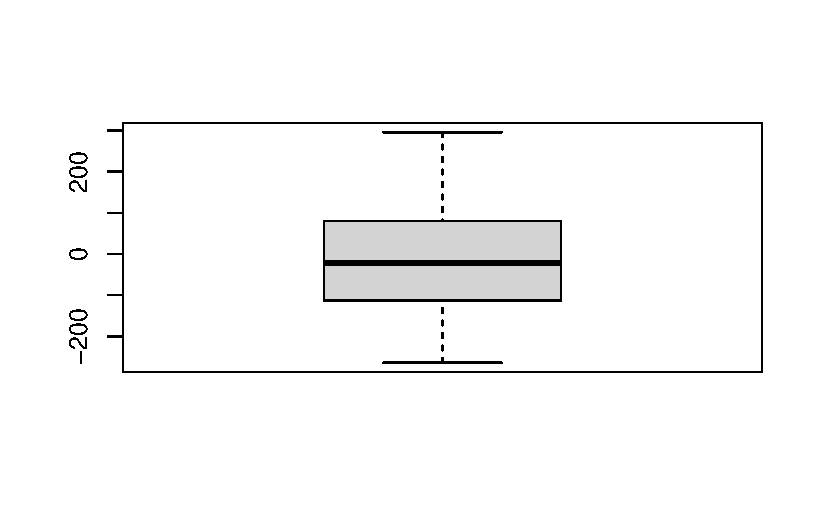
\includegraphics{sta9700_herlan_ch6_2023_04_12_files/figure-pdf/unnamed-chunk-8-1.pdf}

}

\end{figure}

\begin{Shaded}
\begin{Highlighting}[]
\FunctionTok{pairs}\NormalTok{(}\SpecialCharTok{\textasciitilde{}}\NormalTok{grocery.lm}\SpecialCharTok{$}\NormalTok{residuals}\SpecialCharTok{+}\NormalTok{grocery.lm}\SpecialCharTok{$}\NormalTok{fitted.values}\SpecialCharTok{+}\NormalTok{X1}\SpecialCharTok{+}\NormalTok{X2}\SpecialCharTok{+}\FunctionTok{I}\NormalTok{(X1}\SpecialCharTok{*}\NormalTok{X2), }\AttributeTok{data =}\NormalTok{ grocery)}
\end{Highlighting}
\end{Shaded}

\begin{figure}[H]

{\centering 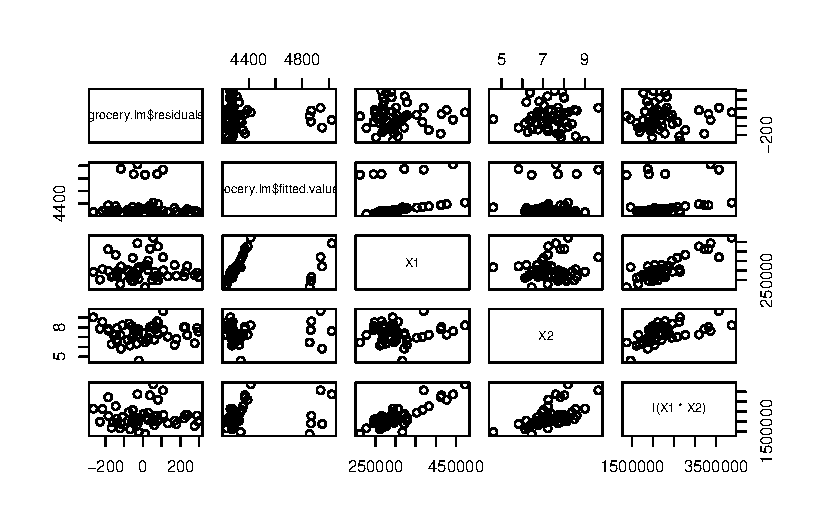
\includegraphics{sta9700_herlan_ch6_2023_04_12_files/figure-pdf/unnamed-chunk-9-1.pdf}

}

\end{figure}

\begin{Shaded}
\begin{Highlighting}[]
\FunctionTok{plot}\NormalTok{(}\FunctionTok{abs}\NormalTok{(grocery.lm}\SpecialCharTok{$}\NormalTok{residuals)}\SpecialCharTok{\textasciitilde{}}\NormalTok{grocery.lm}\SpecialCharTok{$}\NormalTok{fitted.values, }\AttributeTok{data =}\NormalTok{ grocery)}
\end{Highlighting}
\end{Shaded}

\begin{figure}[H]

{\centering 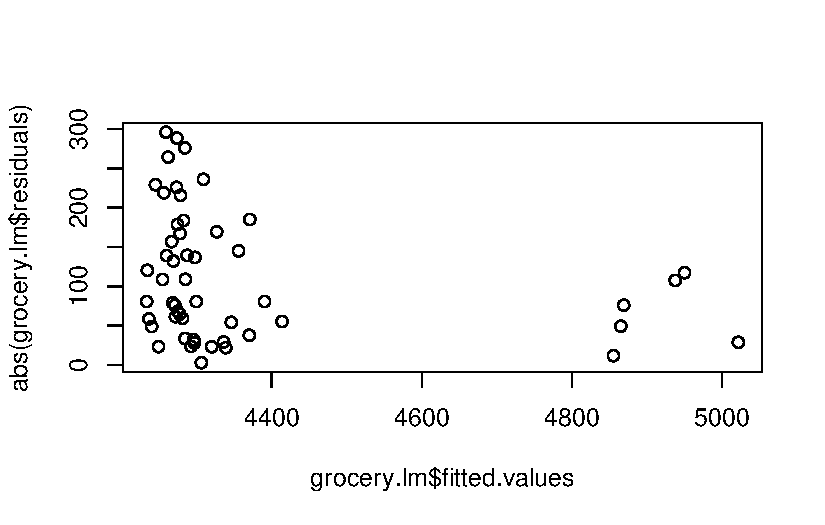
\includegraphics{sta9700_herlan_ch6_2023_04_12_files/figure-pdf/unnamed-chunk-10-1.pdf}

}

\end{figure}

\textbf{c.} Plot the residuals against \(\hat Y\), \(X_{1}\), \(X_{2}\),
\(X_{3}\), and \(X_{1}X_{2}\) on separate graphs. Also prepare a normal
probability plot. Interpret the plots and summarize your findings.

\begin{Shaded}
\begin{Highlighting}[]
\FunctionTok{par}\NormalTok{(}\AttributeTok{mfrow =} \FunctionTok{c}\NormalTok{(}\DecValTok{2}\NormalTok{, }\DecValTok{2}\NormalTok{))}
\FunctionTok{plot}\NormalTok{(grocery.lm)}
\end{Highlighting}
\end{Shaded}

\begin{figure}[H]

{\centering 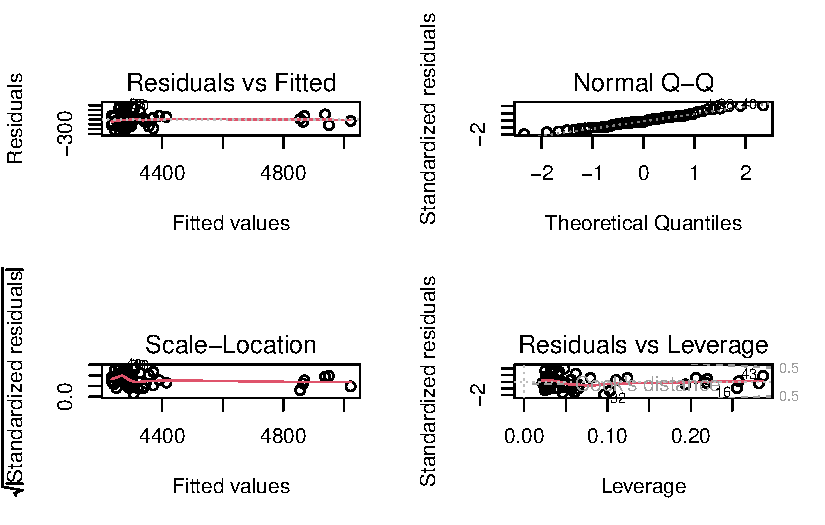
\includegraphics{sta9700_herlan_ch6_2023_04_12_files/figure-pdf/unnamed-chunk-11-1.pdf}

}

\end{figure}

\begin{Shaded}
\begin{Highlighting}[]
\FunctionTok{qqnorm}\NormalTok{(grocery.lm}\SpecialCharTok{$}\NormalTok{residuals) }
\FunctionTok{qqline}\NormalTok{(grocery.lm}\SpecialCharTok{$}\NormalTok{residuals)}
\end{Highlighting}
\end{Shaded}

\begin{figure}[H]

{\centering 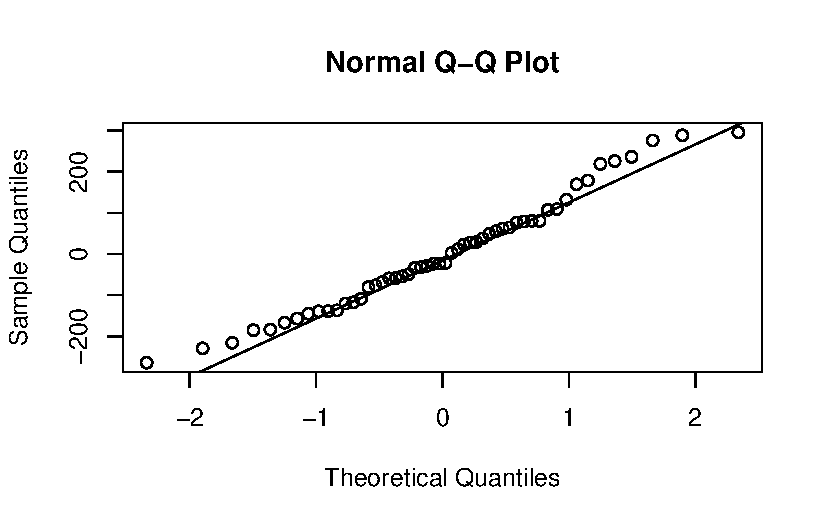
\includegraphics{sta9700_herlan_ch6_2023_04_12_files/figure-pdf/unnamed-chunk-12-1.pdf}

}

\end{figure}

\begin{Shaded}
\begin{Highlighting}[]
\FunctionTok{shapiro.test}\NormalTok{(grocery.lm}\SpecialCharTok{$}\NormalTok{residuals)}
\end{Highlighting}
\end{Shaded}

\begin{verbatim}

    Shapiro-Wilk normality test

data:  grocery.lm$residuals
W = 0.97575, p-value = 0.3644
\end{verbatim}

\begin{Shaded}
\begin{Highlighting}[]
\FunctionTok{lillie.test}\NormalTok{(grocery.lm}\SpecialCharTok{$}\NormalTok{residuals)}
\end{Highlighting}
\end{Shaded}

\begin{verbatim}

    Lilliefors (Kolmogorov-Smirnov) normality test

data:  grocery.lm$residuals
D = 0.08161, p-value = 0.5245
\end{verbatim}

\textbf{d.} Prepare a time plot of the residuals. Is there any
indication that the error term are correlated?

\begin{Shaded}
\begin{Highlighting}[]
\NormalTok{grocery.resid }\OtherTok{\textless{}{-}} \FunctionTok{resid}\NormalTok{(grocery.lm)}
\end{Highlighting}
\end{Shaded}

\begin{Shaded}
\begin{Highlighting}[]
\NormalTok{grocery.resid}
\end{Highlighting}
\end{Shaded}

\begin{verbatim}
          1           2           3           4           5           6 
 -32.063483  169.205091  -21.825426  -54.119552   75.933724   28.000660 
          7           8           9          10          11          12 
-156.684401 -166.983381 -136.691019  275.783546  132.059842  -33.540598 
         13          14          15          16          17          18 
 -59.173782 -215.535629   22.975644 -117.076677  178.568096  -75.863154 
         19          20          21          22          23          24 
 108.947943 -183.565972  -49.165210   11.662167 -120.279732   80.569854 
         25          26          27          28          29          30 
  48.807558  -23.519661   78.869281  -58.398630   61.303251  -23.214763 
         31          32          33          34          35          36 
-138.978271 -264.053024  218.752742  235.960794 -229.055311  -67.763118 
         37          38          39          40          41          42 
-139.284659  288.397234 -108.609359  295.751820   29.065887   80.555515 
         43          44          45          46          47          48 
 107.399309   55.197555   37.772702  -80.508888 -144.901536  -28.753312 
         49          50          51          52 
   2.731302  225.697849 -184.877629   64.516810 
\end{verbatim}

\begin{Shaded}
\begin{Highlighting}[]
\FunctionTok{plot}\NormalTok{(grocery}\SpecialCharTok{$}\NormalTok{X1, grocery.resid, }
     \AttributeTok{ylab =} \StringTok{"Residuals"}\NormalTok{, }\AttributeTok{xlab =} \StringTok{"X1"}\NormalTok{, }
     \AttributeTok{main =} \StringTok{"Grocery"}\NormalTok{) }
\FunctionTok{abline}\NormalTok{(}\DecValTok{0}\NormalTok{, }\DecValTok{0}\NormalTok{)                  }\CommentTok{\# the horizon}
\end{Highlighting}
\end{Shaded}

\begin{figure}[H]

{\centering 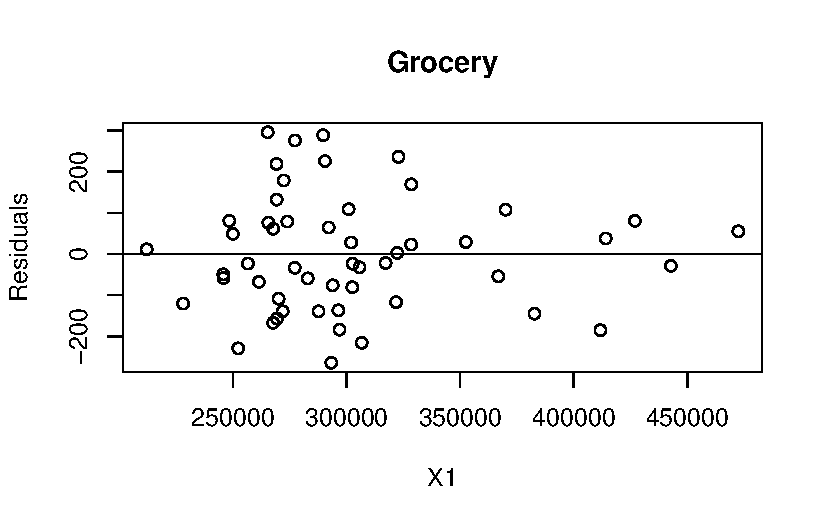
\includegraphics{sta9700_herlan_ch6_2023_04_12_files/figure-pdf/unnamed-chunk-17-1.pdf}

}

\end{figure}

\begin{Shaded}
\begin{Highlighting}[]
\FunctionTok{plot}\NormalTok{(grocery}\SpecialCharTok{$}\NormalTok{X2, grocery.resid, }
     \AttributeTok{ylab =} \StringTok{"Residuals"}\NormalTok{, }\AttributeTok{xlab =} \StringTok{"X2"}\NormalTok{, }
     \AttributeTok{main =} \StringTok{"Grocery"}\NormalTok{) }
\FunctionTok{abline}\NormalTok{(}\DecValTok{0}\NormalTok{, }\DecValTok{0}\NormalTok{)                  }\CommentTok{\# the horizon}
\end{Highlighting}
\end{Shaded}

\begin{figure}[H]

{\centering 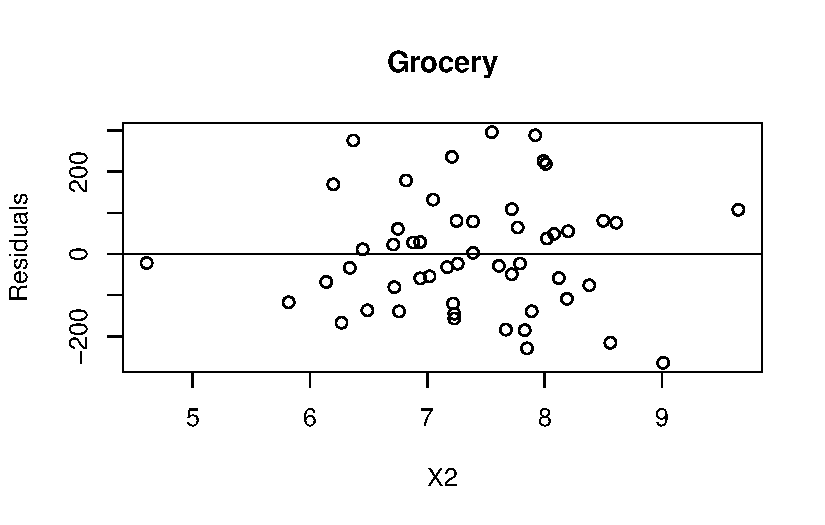
\includegraphics{sta9700_herlan_ch6_2023_04_12_files/figure-pdf/unnamed-chunk-18-1.pdf}

}

\end{figure}

\begin{Shaded}
\begin{Highlighting}[]
\FunctionTok{plot}\NormalTok{(grocery}\SpecialCharTok{$}\NormalTok{X2, grocery.resid, }
     \AttributeTok{ylab =} \StringTok{"Residuals"}\NormalTok{, }\AttributeTok{xlab =} \StringTok{"X3"}\NormalTok{, }
     \AttributeTok{main =} \StringTok{"Grocery"}\NormalTok{) }
\FunctionTok{abline}\NormalTok{(}\DecValTok{0}\NormalTok{, }\DecValTok{0}\NormalTok{)                  }\CommentTok{\# the horizon}
\end{Highlighting}
\end{Shaded}

\begin{figure}[H]

{\centering 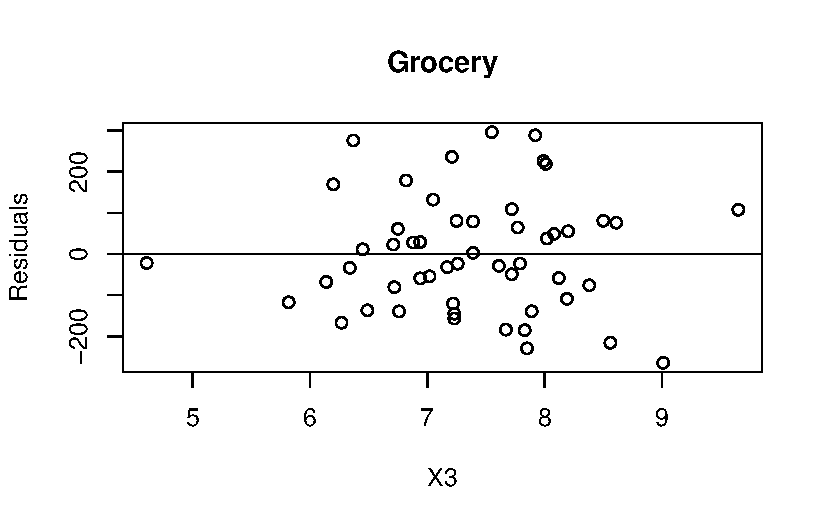
\includegraphics{sta9700_herlan_ch6_2023_04_12_files/figure-pdf/unnamed-chunk-19-1.pdf}

}

\end{figure}

\emph{6.11}

\emph{a.} Test whether there is a regression relation, using level of
significance 0.05. State the alternatives, decision rule, and
conclusion. What does your result imply \(B_{1}\), \(B_{2}\), and
\(B_{3}\)? What is the \(P\)-value of the test?

\begin{Shaded}
\begin{Highlighting}[]
\FunctionTok{summary}\NormalTok{(grocery.lm)}
\end{Highlighting}
\end{Shaded}

\begin{verbatim}

Call:
lm(formula = Y ~ X1 + X2 + X3, data = grocery)

Residuals:
    Min      1Q  Median      3Q     Max 
-264.05 -110.73  -22.52   79.29  295.75 

Coefficients:
              Estimate Std. Error t value Pr(>|t|)    
(Intercept)  4.150e+03  1.956e+02  21.220  < 2e-16 ***
X1           7.871e-04  3.646e-04   2.159   0.0359 *  
X2          -1.317e+01  2.309e+01  -0.570   0.5712    
X3           6.236e+02  6.264e+01   9.954 2.94e-13 ***
---
Signif. codes:  0 '***' 0.001 '**' 0.01 '*' 0.05 '.' 0.1 ' ' 1

Residual standard error: 143.3 on 48 degrees of freedom
Multiple R-squared:  0.6883,    Adjusted R-squared:  0.6689 
F-statistic: 35.34 on 3 and 48 DF,  p-value: 3.316e-12
\end{verbatim}

\begin{Shaded}
\begin{Highlighting}[]
\FunctionTok{Anova}\NormalTok{(grocery.lm, }\AttributeTok{type =} \StringTok{\textquotesingle{}III\textquotesingle{}}\NormalTok{)}
\end{Highlighting}
\end{Shaded}

\begin{verbatim}
Anova Table (Type III tests)

Response: Y
             Sum Sq Df  F value    Pr(>F)    
(Intercept) 9245215  1 450.2861 < 2.2e-16 ***
X1            95707  1   4.6614   0.03588 *  
X2             6675  1   0.3251   0.57123    
X3          2034514  1  99.0905 2.941e-13 ***
Residuals    985530 48                       
---
Signif. codes:  0 '***' 0.001 '**' 0.01 '*' 0.05 '.' 0.1 ' ' 1
\end{verbatim}

\(H_{0}\): \(B_{1}\) = \(B_{2}\) = \(B_{3}\)

\(H_{a}\): not all \(B_{k}\) = 0 (\emph{k} = 1, 2, 3).

\(MSR\) = 725,535

\(MSE\) = 20,531

\(F^{*}\) = 725,535/531.9 = 35.337

\(F(0.95; 3, 48)\) = 2.79806.

If \(F^{*}\) \textless{} 2.79806 conclude \(H_{0}\), otherwise
\(H_{a}\).

Conclude \(H_{a}\). \(P\)-value = \textless{} 0.05.

\textbf{b.} Estimate \(B_{1}\) and \(B_{3}\) jointly by the Bonferroni
procedure, using a 95 percent family confidence coefficient. Interpret
your result.

\begin{Shaded}
\begin{Highlighting}[]
\FunctionTok{confint.lm}\NormalTok{(grocery.lm)}
\end{Highlighting}
\end{Shaded}

\begin{verbatim}
                    2.5 %       97.5 %
(Intercept)  3.756677e+03 4.543098e+03
X1           5.409544e-05 1.520065e-03
X2          -5.959506e+01 3.326302e+01
X3           4.976064e+02 7.495025e+02
\end{verbatim}

\textbf{c.} Calculate the coefficient of multiple determination
\(R^{2}\). How is this measure interpreted here?

\begin{Shaded}
\begin{Highlighting}[]
\FunctionTok{summary}\NormalTok{(grocery.lm)}
\end{Highlighting}
\end{Shaded}

\begin{verbatim}

Call:
lm(formula = Y ~ X1 + X2 + X3, data = grocery)

Residuals:
    Min      1Q  Median      3Q     Max 
-264.05 -110.73  -22.52   79.29  295.75 

Coefficients:
              Estimate Std. Error t value Pr(>|t|)    
(Intercept)  4.150e+03  1.956e+02  21.220  < 2e-16 ***
X1           7.871e-04  3.646e-04   2.159   0.0359 *  
X2          -1.317e+01  2.309e+01  -0.570   0.5712    
X3           6.236e+02  6.264e+01   9.954 2.94e-13 ***
---
Signif. codes:  0 '***' 0.001 '**' 0.01 '*' 0.05 '.' 0.1 ' ' 1

Residual standard error: 143.3 on 48 degrees of freedom
Multiple R-squared:  0.6883,    Adjusted R-squared:  0.6689 
F-statistic: 35.34 on 3 and 48 DF,  p-value: 3.316e-12
\end{verbatim}



\end{document}
